
\chapter{Building Thermal Expansion Measurement System
and its interfacing} 
\label{Appendix A}

\section{Building Thermal Expansion Measurement System
and its interfacing}
\subsection{The principle of measurement system}
The coefficient of linear Thermal expansion ($\alpha$) denotes the change in length of the given
material when heated. It is a material property and the same may be written as, $$\alpha = \frac{\frac{L_{f}-L_{0}}{L_{0}}}{T_{f}-T_{0}}$$
The quantity is of high significance for studying the thermal properties of materials for
fundamental as well as applied areas. A couple of methods have been reported for the measurement of TEC. Those can be broadly classified
as-
\begin{itemize}
    \item Interferometry - light interference based
    \item Diletometry
    \item Capacitance based
    \item LVDT-based
\end{itemize}
In the case of interferometric methods, the sample surface is shone with a monochromatic light beam, and the interference fringes are observed from the rays reflected on the surface. Although this method has high precision, it is applicable to only a limited range of $\alpha$ values and depends on the sample surface optical properties.\\
On the other hand, in dilatometric methods, the change in length of the material is measured by means of a linear translation rod/arm assembly that changes the signal on the capacitance bridge or an LVDT, respectively. We have developed a system based on this method using a Linear Variable Differential Transformer (LVDT) as a linear transducer.
\subsection{Instrumentation}
The entire system is home built and the schematic diagram of the system is shown in Fig 2.8. 
\begin{figure}
    \centering
    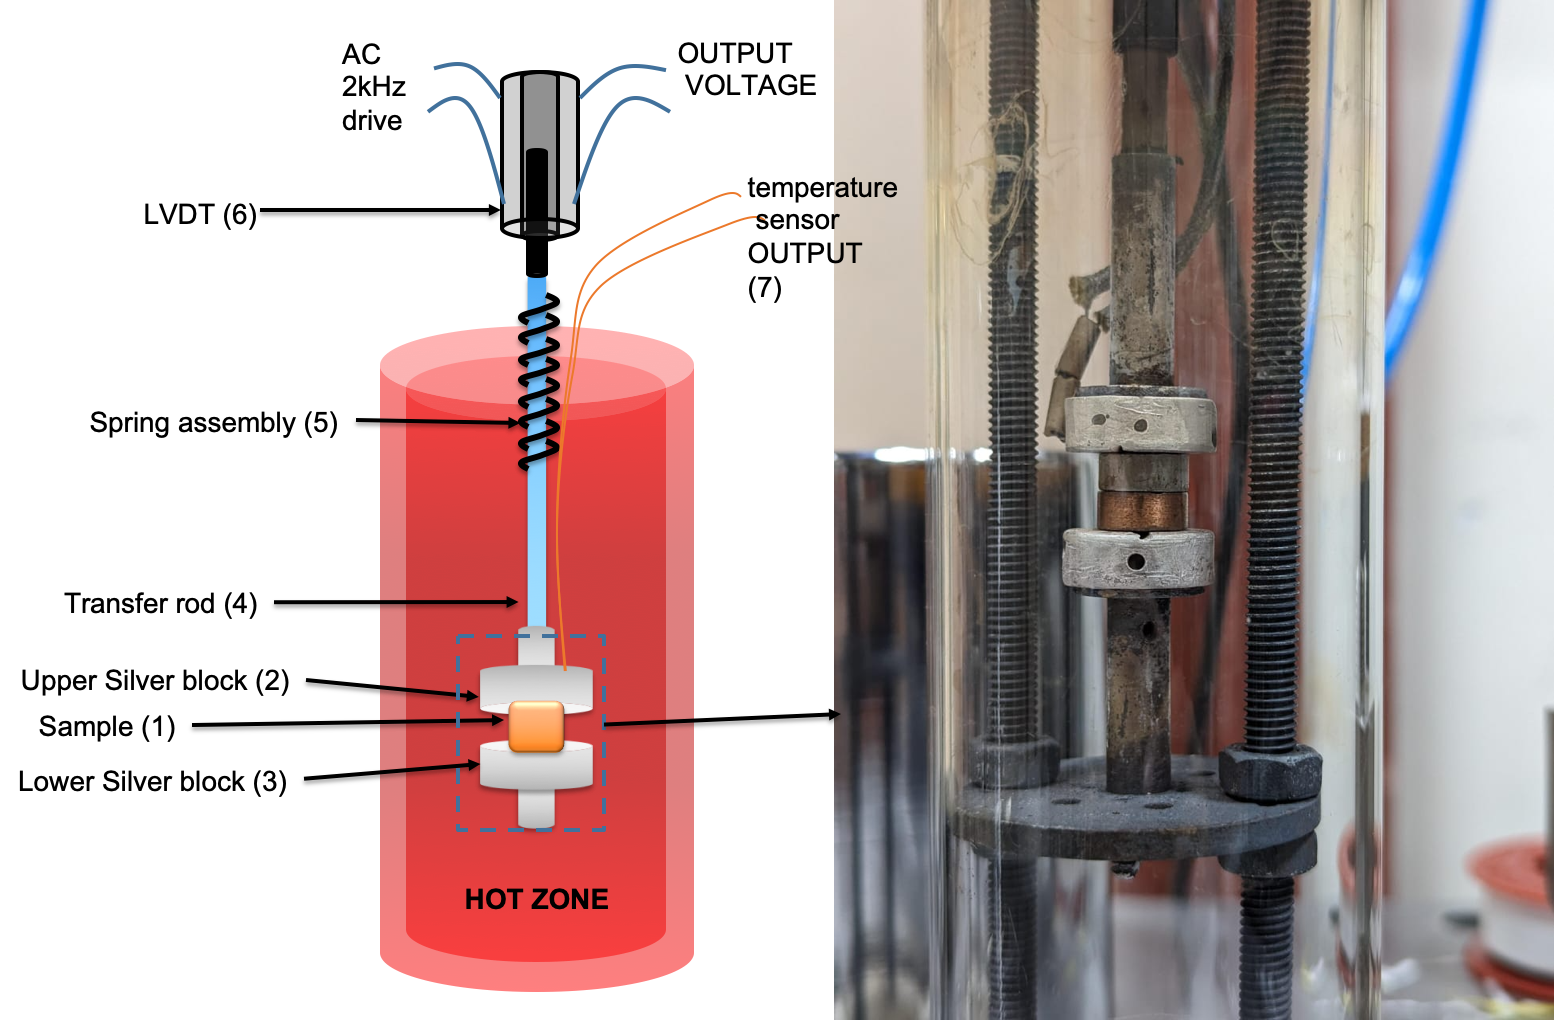
\includegraphics[width=1\linewidth]{Thesis Prashant//Images//media/image9.png}
    \caption{The schematic diagram of the home built Thermal expansion measurement system and its digital
photograph.}
    \label{fig:enter-label}
\end{figure}
The sample (1) to be measured is sandwiched between two silver metal blocks (2 and 3) for to hold in place, as well as silver helps in better temperature equilibration. The lower silver block is fixed while the upper silver block is mounted on a transfer rod/arm (4) which is made up of steel (not modified to Quartz). For this top silver block to always press against the sample, it is equipped with a spring assembly (5) that always pushes it against the sample. This ensures that
any change is sample length is directly translated to the other end of the rod where the transducer is place. As mentioned above, LVDT is used here as a transducer as shown in the figure.
The enlarged view of sample holder assembly is also shown in Fig 1. The entire sample
holder goes inside a vacuum chamber made of the quartz tube with suitable couplers and flanges.
The Quartz tube is inserted into the furnace (hot zone) to raise the sample temperature uniformly.
A k-type thermocouple is inserted in upper silver block to measure the sample temperature. The
electronic components are place away from the hot zone. If the sample is placed, it is expected to show a certain signal from the LVDT arm. If its temperature is raised and it expands the change is length of the sample caused the quartz rod to
push the core of LVDT further inside producing a change in signal.

\subsubsection{Design and working of LVDT}
An AC power source of 1.2 V at 2 kHz sine wave was used to power the LVDT, and a Keithley
2700 Multi-meter cum data acquisition system was used to read its analog outputs.
\begin{figure}
    \centering
    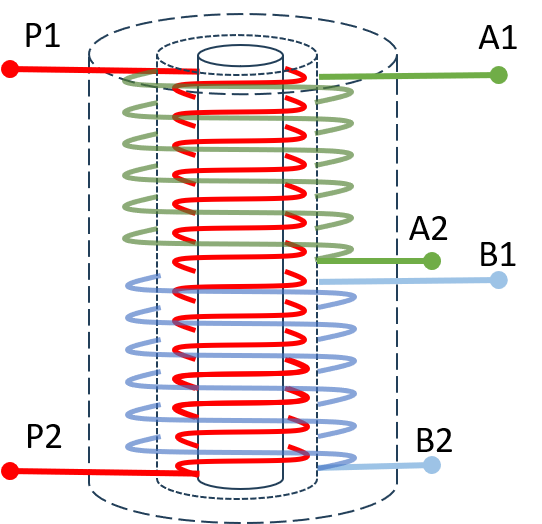
\includegraphics[width=0.5\linewidth]{Thesis Prashant//Images//media/image10.png}
    \caption{Circuit diagram of LVDT primary winding and Secondary winding.}
    \label{fig:enter-label}
\end{figure}
A hollow cylinder of insulating material serves as its main component. This insulating cylinder has one main winding P and two secondary winding A and B looped around its circumference. In the middle of the insulating cylinder lies the main winding P, and on either side of it are two secondary winding, A and B, coiled in complete opposition to one another as shown in Fig 2.9 In other words, A and B are moving in opposite directions. A magnetic or armature core is put within the insulating hollow cylinder and can move freely in both directions. Attaching the soft iron core to the object under study allows for the measurement of displacement. Nickel is commonly used in soft-core because of its great sensitivity. [9]
\begin{figure}
    \centering
    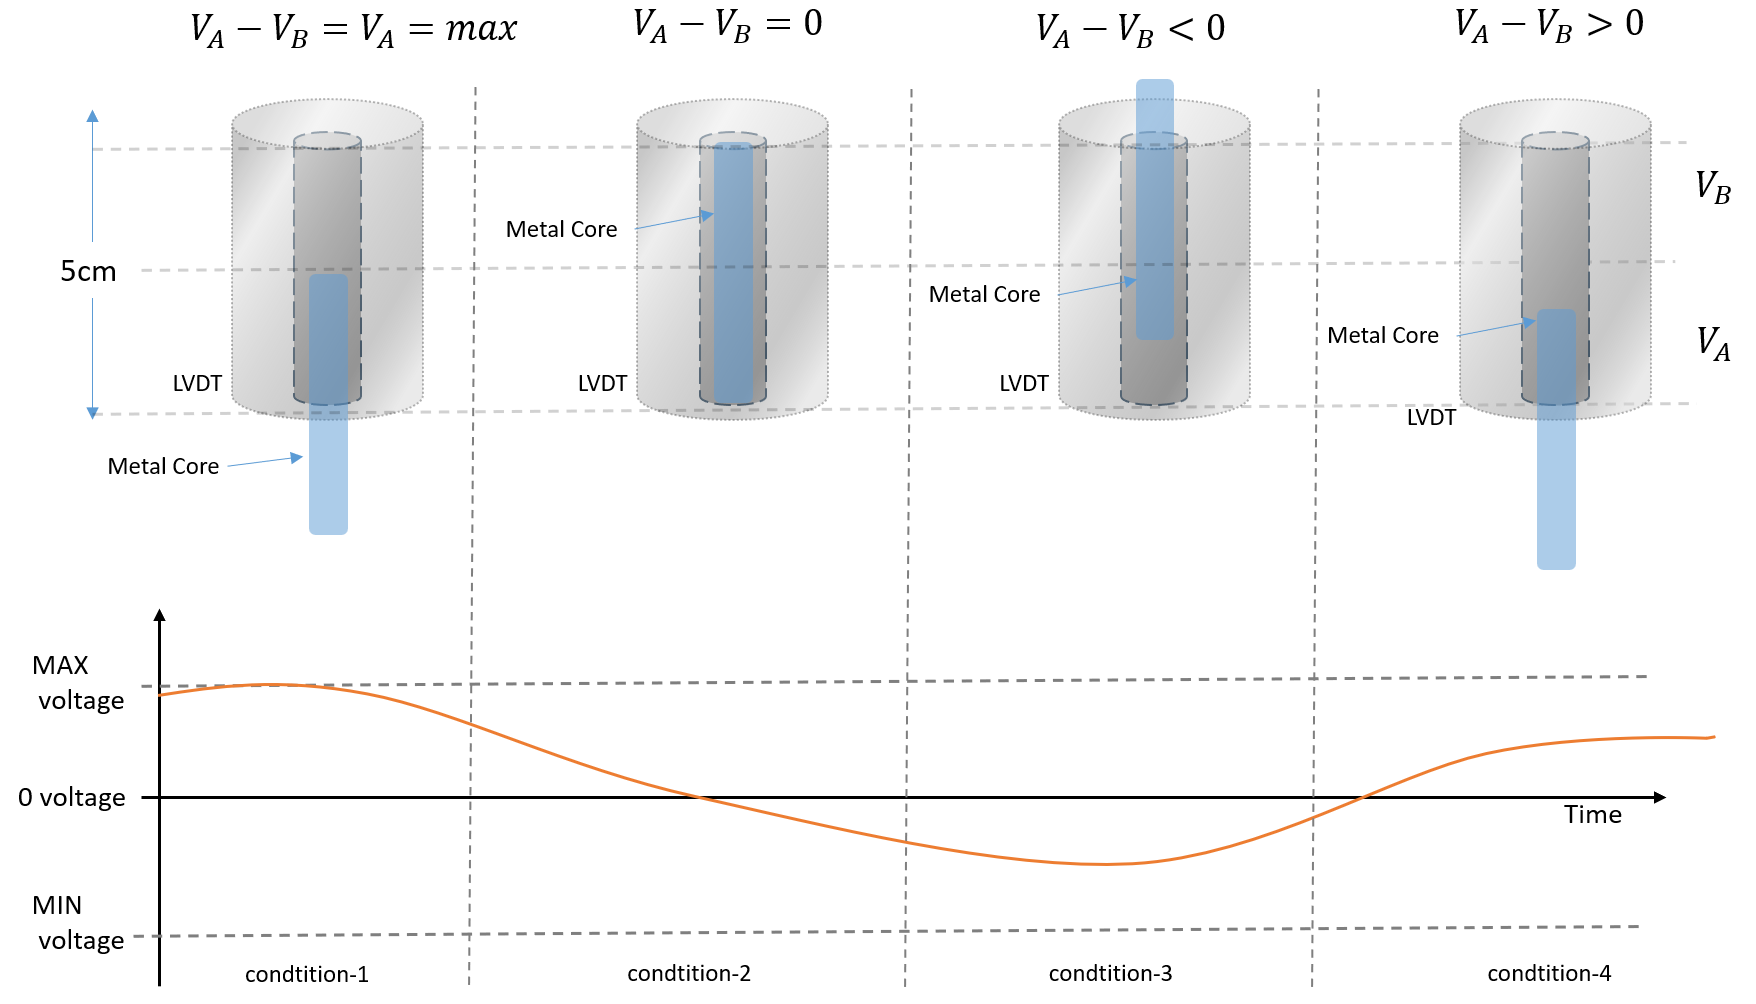
\includegraphics[width=0.8\linewidth]{Thesis Prashant//Images//media/image11.png}
    \caption{Different placements of metal core inside LVDT and corresponding voltage signal
being generated.}
    \label{fig:enter-label}
\end{figure}

From Faraday’s law of electromagnetic induction, an EMF is produced in the secondary winding. When the primary winding is supplied with an alternating current, a magnetic flux is generated that travels through both A and B. Primary winding flux is proportional to secondary winding conductor count. The primary coil is powered using an AC signal (here we used 2 kHz and 1.2 V). The magnetic induction into the secondary develops due to magnetic core placed in between (like a transformer). When the core of LVDT may slide to shifts to top, bottom or to the null position. There will be an increase or decrease in the output difference. In this case, the LVDT's output voltage is a linear function of core displacement up
to a certain point (5 mm from the LVDT's null position limit). This graph displays the variation in output voltage versus displacement. (See Fig 2.10 ).

Measuring TEC requires monitoring the output voltage of the LVDT that changes when the temperature of the sample under consideration varies. With increment in temperature, material expands and so the connected shaft to the metal core inside LVDT moves, which gives change in voltage proportional to the change in position of the metal core. Therefore, LVDTs can
be consider as length or position sensors that detect changes in length or position.

In order to measure the TEC a change in length of material with change of temperature is to be measured, and initial length of the sample should be known. With a good sensitive LVDT even a small expansion (sub mm) can also be measured accurately. Thus, the final system measurement should give the plot between change in length vs temperature. Change in length becomes change in Voltage by using LVDT’s sensitivity factor (typically given in mV/mm).

Let $V_{A}$ and $V_{B}$ be the voltages produced by the A and B coil, respectively. Since A and B are connected in opposite directions, they must be connected in series to create a single voltage with a phase difference of 180 degrees. Because of this, the secondary coil's output will be the difference between the two voltages produced by the device.
$$V = V_{A}-V_{B}$$
The secondary coil’s voltage output is linear for small displacements, as seen in Fig 12. There are no discrete steps in the voltage output, and the resolution is more a function of the testing apparatus than the transducer itself. No further intermediary amplifiers are required since the output voltage is large and easily measurable. The transducer can withstand significant vibration and stress because of its high sensitivity. Most importantly, the measuring system is insensitive to changes in temperature and suffers no loss due to friction. This attribute is necessary because of its proximity to a high-temperature furnace.

\subsection{Calibration and Measurement}
\textbf{Fig13}--- The preliminary measurements performed with the system are shown in Fig. The system
\begin{figure}
    \centering
    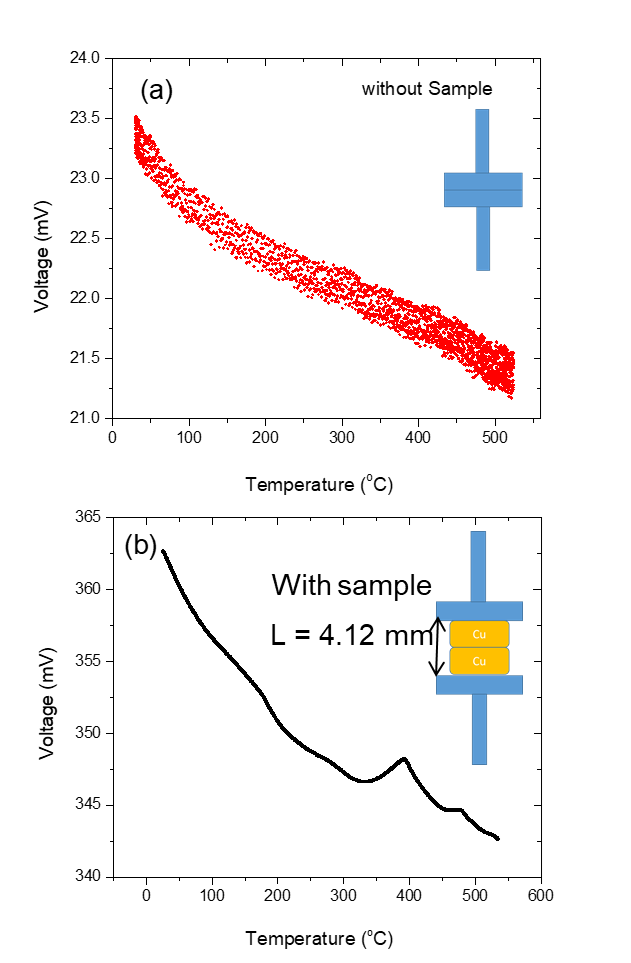
\includegraphics[width=0.5\linewidth]{Thesis Prashant//Images//media/image12.png}
    \caption{(a) Without and (b) With sample thermal expansion measurement data. Two Cu
samples in the stack (each with L = 4.12mm) were used as samples.}
    \label{fig:enter-label}
\end{figure}
background data was measured without any sample and shown in Fig (a). because of the
component used for sample holder there were non-zero background signal measured. Because
of its low value there is a significant noise in the background. Similarly, the data was also
measured by placing a sufficiently long Cu sample(s) between the two silver holders. This
yielded about one order of magnitude large change in the voltage. Cu is used here for
standardization for its known and high value of TEC. 
Nevertheless, there are several non-monotonous changes in the voltage that are not expected.

\begin{figure}
    \centering
    
\includegraphics[width=0.8\linewidth]{Thesis Prashant//Images//media/image13.png}
    \caption{Measurements performed on the (a) same Cu sample, L= 4.12mm and (b) longer sample (8.04
mm length Cu sample)}
    \label{fig:enter-label}
\end{figure}
Further, optimization of the system needs dynamic measurements. Also, the
final data is to be represented as ΔL/L. Here, copper has very high thermal expansion coefficient. However, for insulating samples like ceramics etc. the TEC value is low and hence the is of the order of background. In that case, it will be challenging to analyze the result when signal to noise ratio is low.

\section{Thermal Expansion Temperature v/s Voltage}

\begin{figure}
    \centering
    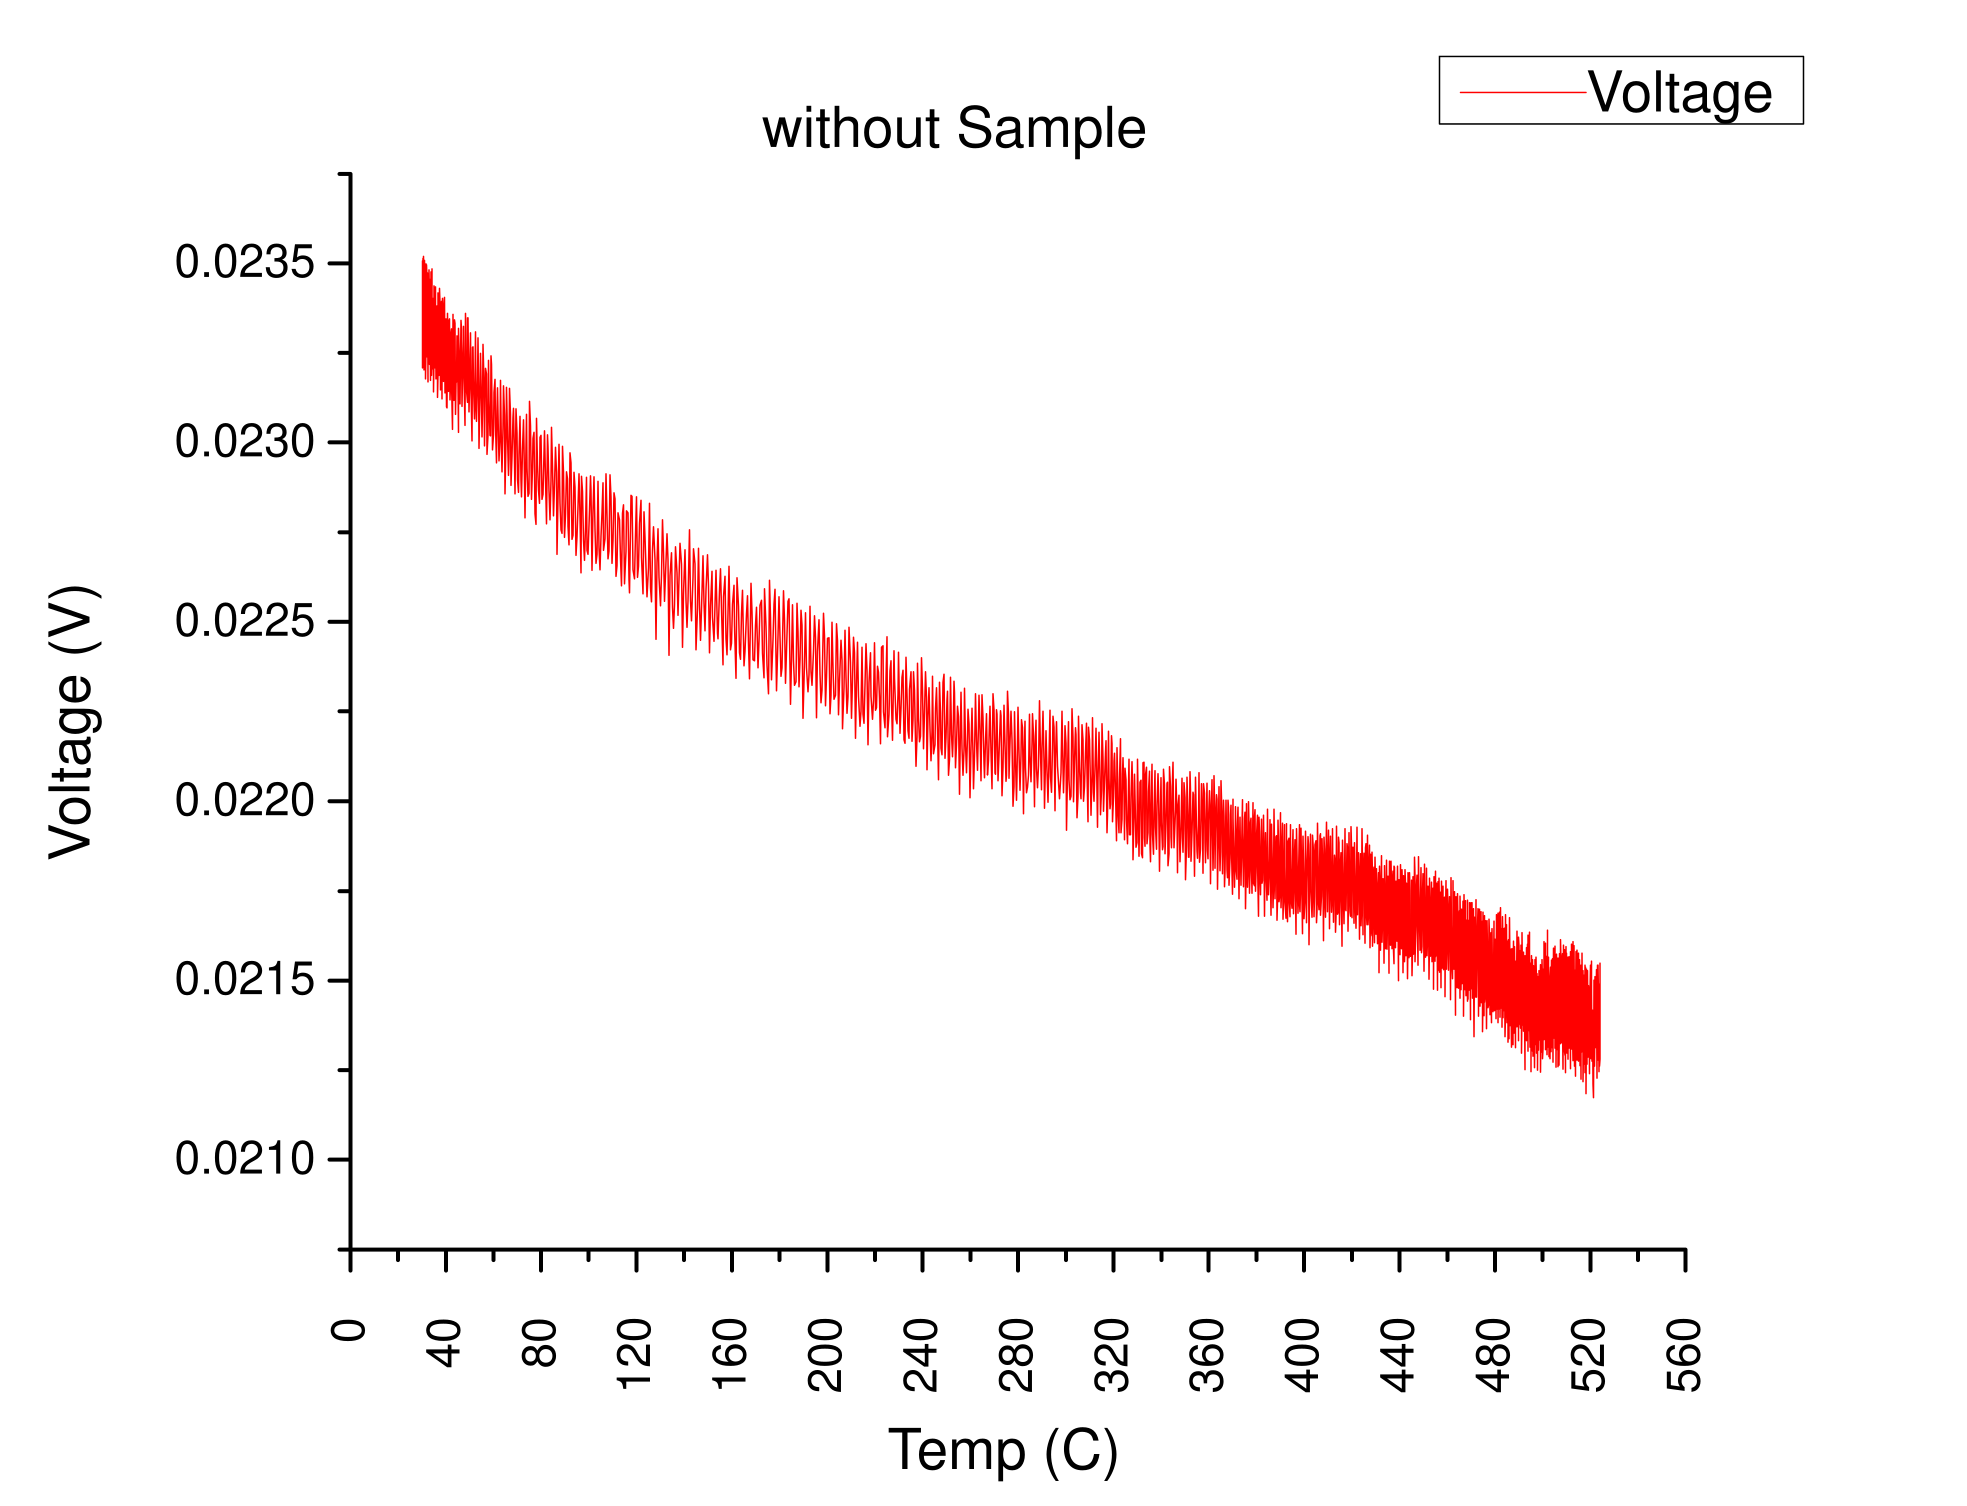
\includegraphics[width=0.6\linewidth]{Thesis Prashant//Images//media/image22.png}
    \caption{without sample thermal expansion measurement}
    \label{fig:enter-label}
\end{figure}
